La aproximación teórica desarrollada por \parencite{DidiHuberman2011}, en diálogo con las contribuciones fundamentales de \parencite{Benjamin2004} y \parencite{Warburg2010}, establece que el acto de observar una imagen genera significados sobre lo observado. Para los propósitos de esta investigación, resulta fundamental delimitar tanto los elementos teóricos como los instrumentales que guiarán la lectura del corpus de imágenes seleccionado. El campo de los estudios visuales proporciona un marco argumentativo robusto para el análisis de imágenes \parencite{Abril2007}. Este enfoque nos permite construir un escenario metodológico sólido desde el cual aproximarnos, con la necesaria sensibilidad visual, al conjunto de discursos visuales, con el objetivo de elaborar escenarios interpretativos coherentes. Este marco teórico define y proyecta los alcances específicos del trabajo analítico con dichas imágenes.


Como señalan \parencite{Perez2010}:
\begin{quote}
Trabajar con imágenes no sólo es muy entretenido, sino que el proceso de encontrarlas y superponerlas es también muy esclarecedor intelectualmente. Muchas veces primero encuentro la imagen y luego escribo el texto que la acompaña. (p. 45)
\end{quote}

El proceso intelectual de esta investigación comienza con la búsqueda y selección de imágenes. Considerando el extenso impacto mediático del caso de crisis y cierre del Hospital San Juan de Dios (HSJD), se ha realizado una cuidadosa selección que contribuye a la definición de categorías de análisis y codificación.

El caso del San Juan resulta emblemático en el contexto de las crisis sociales e institucionales derivadas de las transformaciones en los sistemas de salud pública, destacándose por su trayectoria histórica como institución hospitalaria fundamental para Bogotá y referente en la medicina suramericana.

La abundante producción investigativa y comunicativa evidencia su relevancia histórica, legando un importante acervo de información sobre aspectos históricos, sociales, políticos, laborales, médicos y pedagógicos. Sin embargo, esta investigación se centra específicamente en las expresiones artísticas como constructoras de sentido. Los registros de obra y enunciados visuales se analizan como evidencias. 

Para delimitar el alcance del trabajo con discursos visuales, es importante precisar que no nos limitaremos a un único tipo de imagen. Como señala el iconólogo W.J.T. \parencite{Mitchell2005}, el término ``imagen'' denota tanto el componente físico u objetual como entidades mentales, memoriales y perceptuales. Aunque las imágenes mentales carecen de materialidad física, tienen existencia en nuestro cuerpo y mente, manifestándose a través del lenguaje en el colectivo social.

Las categorías de análisis para las imágenes artísticas relacionadas con la crisis del HSJD incluyen conceptos como: imagen-síntoma, imagen-malicia, imagen-combate, imagen-aura, imagen-fantasma \parencite{DidiHuberman2011}; imagen-virtual, imagen-digital \parencite{Manovich2005}; imagen-dialéctica \parencite{Benjamin2004}; e imagen-tiempo, imagen-movimiento, imagen-recuerdo, imagen-sueño \parencite{Deleuze1985}.

Este estudio busca enfoques alternativos a la descripción iconográfica, incorporando la búsqueda del anacronismo y el malestar en las imágenes, \textit{el síntoma}.

\begin{quote}
    Sería necesario, pues, interrogarse también sobre lo que quiere decir, sobre lo que implica la palabra “síntoma”. Palabra difícil de delimitar: no designa una cosa aislada, ni incluso un proceso reductible a uno o dos vectores, o a un número preciso de componentes. Es una complejidad de segundo grado. No es lo mismo que un concepto semiológico o clínico, incluso cuando compromete una determinada comprensión de la emergencia (fenoménica) del sentido, e incluso si compromete una determinada comprensión de la pregnancia (estructural) de la disfuncionalidad. Esta noción denota por lo menos una doble paradoja, visual y temporal, cuyo interés resulta comprensible para nuestro campo de interrogación sobre las imágenes y el tiempo. \parencite[p. 63]{DidiHuberman2011}
\end{quote}

\begin{figure}[h!]
    \centering
    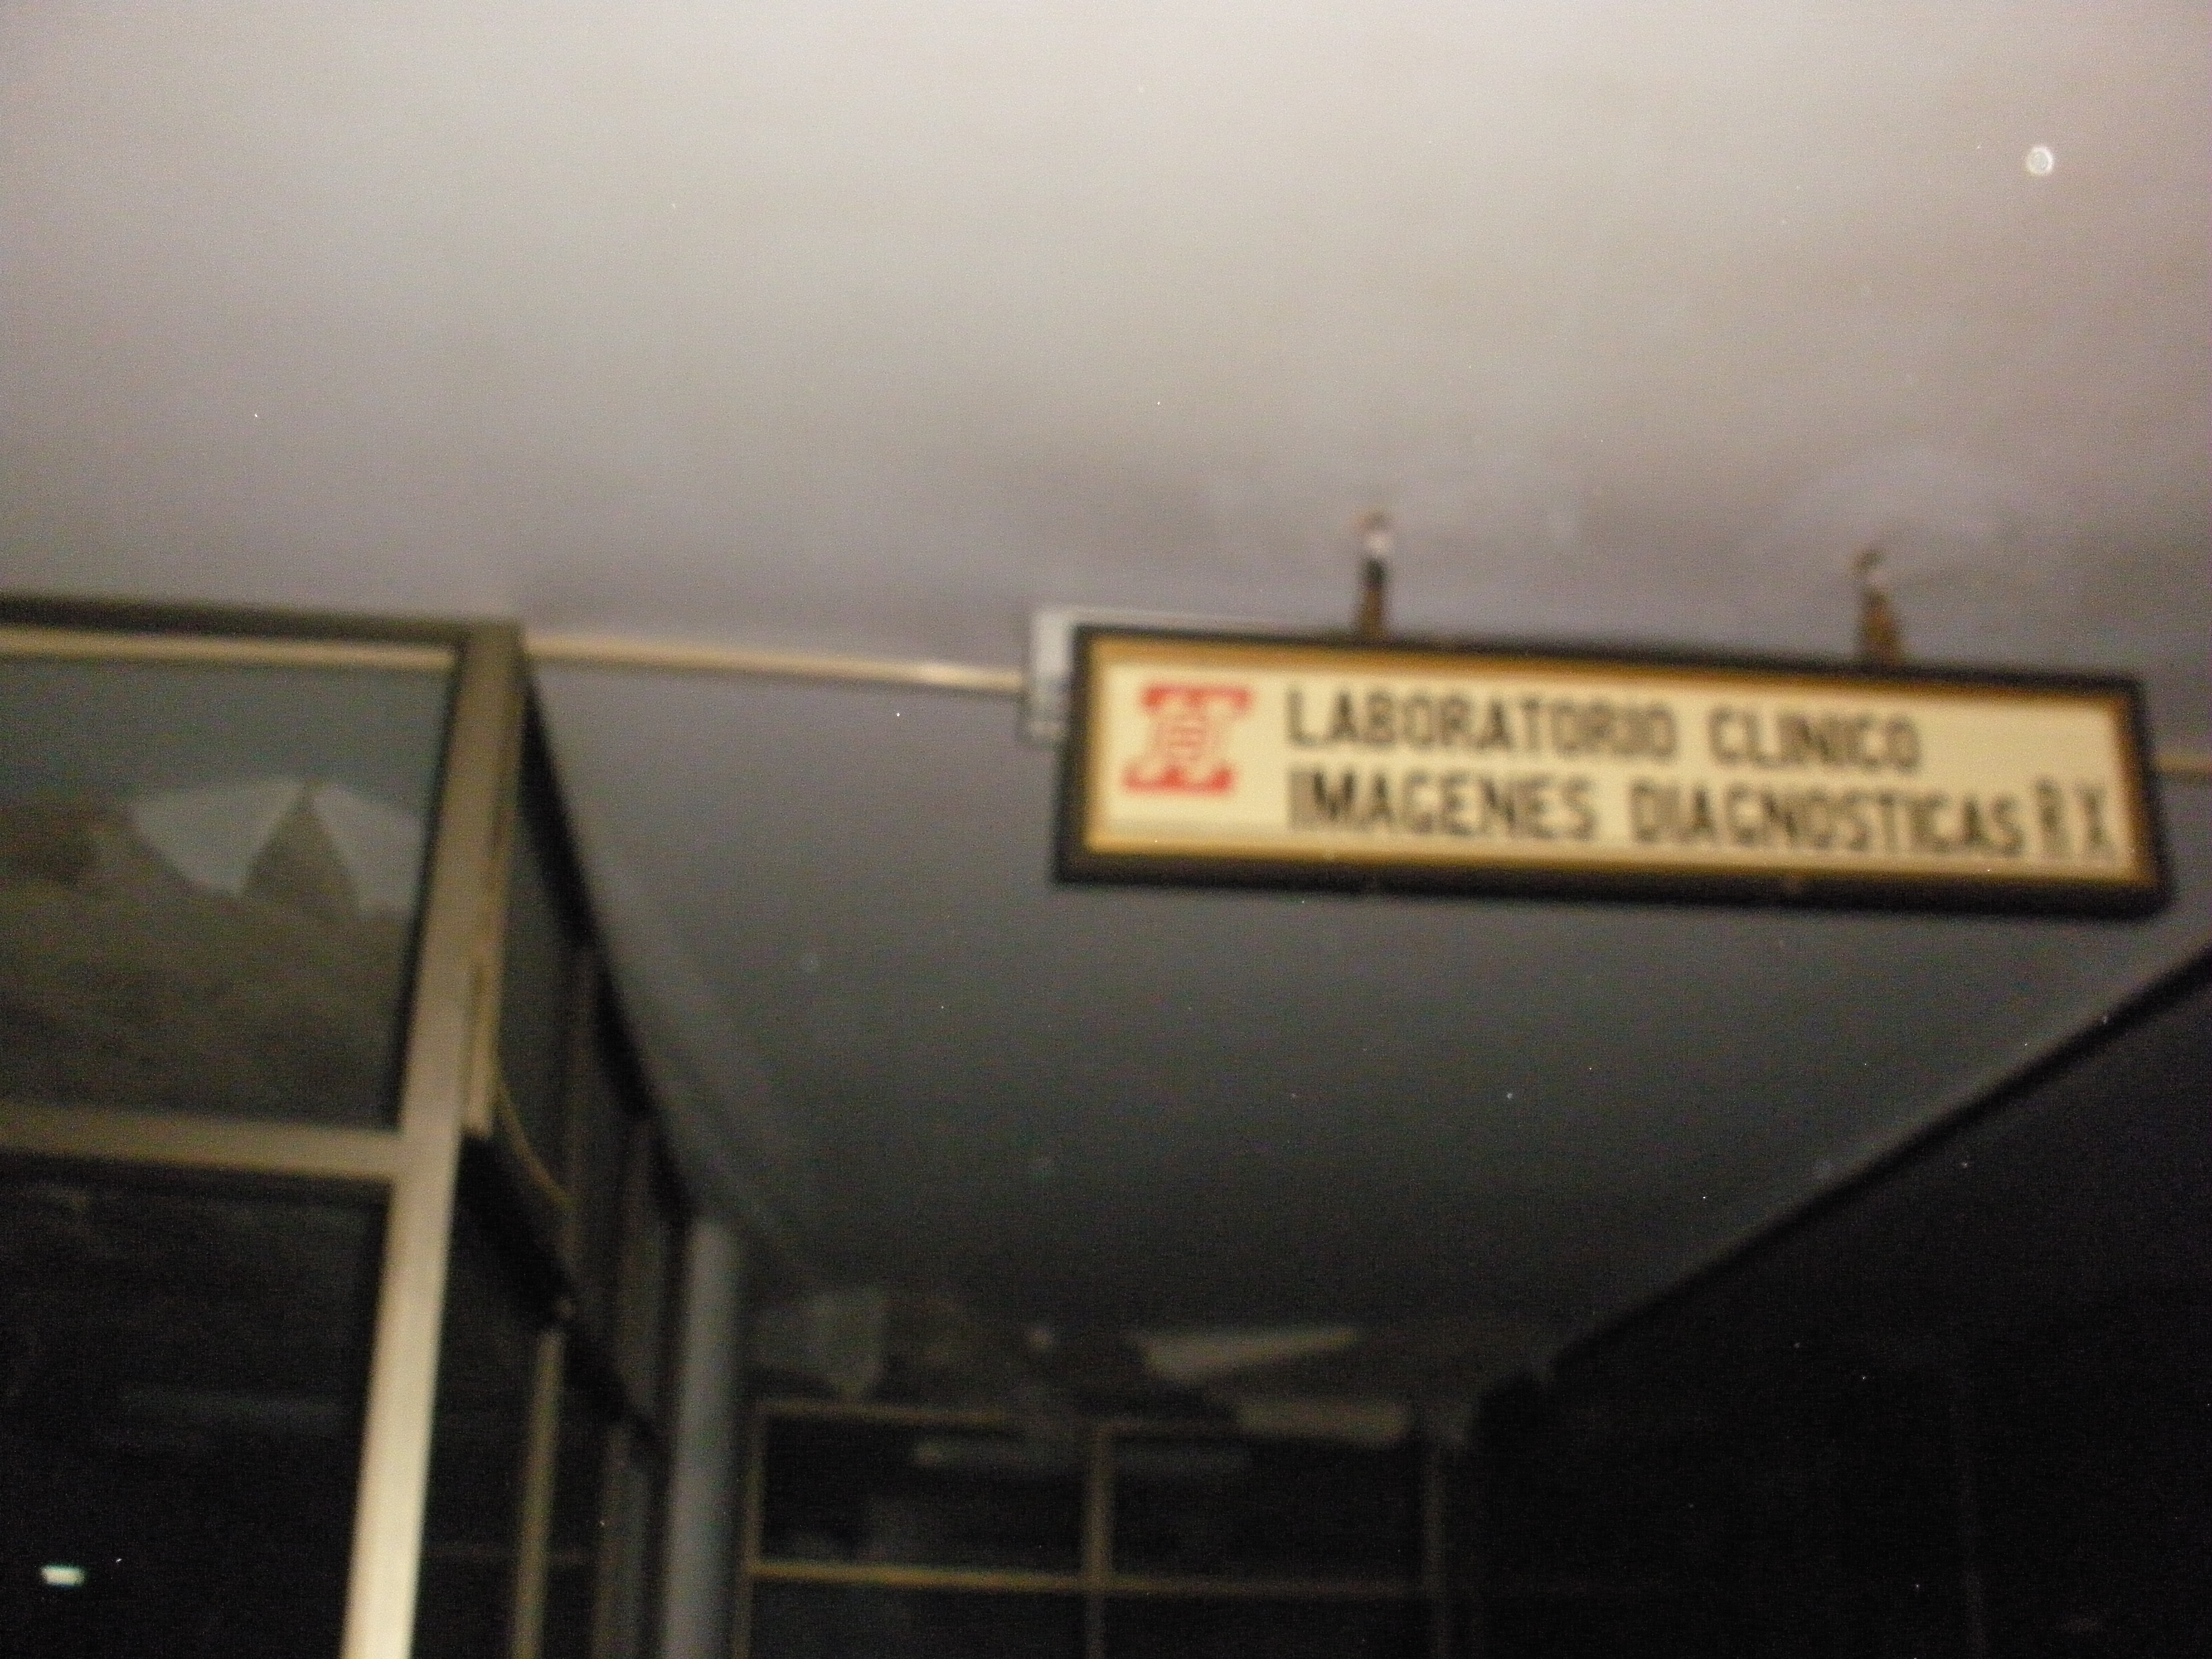
\includegraphics[width=\textwidth]{P7260115.jpg}
    \caption{Señalética imágenes diagnósticas. Foto: Archivo de Margarita Castro.}
    \label{fig:senaletica_imagenes_diagnosticas}
\end{figure}

La investigación se propone profundizar en las relaciones de sentido entre la realidad social y vital del Hospital San Juan de Dios (HSJD) a través del análisis del malestar subyacente en los registros de obra y fotografías testimoniales. Este análisis buscará aplicaciones metodologógicas en dos conceptos teóricos clave: el \textit{montaje}, desarrollado por \parencite{Benjamin2004}, y la noción de \textit{supervivencia} propuesta por \parencite{Warburg2010}. La articulación de estos conceptos permite activar las latencias y síntomas de la memoria social mediante la experiencia visual del observador. Con esta postura investigativa se adopta el pensamiento a través de imágenes y sus vehículos: los objetos materiales, los medios virtuales y la imaginación.

\begin{quote}
    Fiction uses imagination as a way of knowing that establishes empathy and intuitively explores the deeper dimensions of events, experiences, and complex human experiences that cannot be fully encapsulated in the literal presentation of facts. \parencite[p. 30]{Leavy2018}
    
    \footnotesize
    (Traducción propia: La ficción utiliza la imaginación como una forma de conocimiento que establece empatía y explora intuitivamente las dimensiones más profundas de los eventos, las experiencias y los complejos aspectos de la condición humana que no pueden ser completamente encapsulados en la presentación literal de los hechos.)
    \normalsize
\end{quote}

\section{Imagen-síntoma}

El análisis de las imágenes artísticas relacionadas con el Hospital San Juan de Dios (HSJD) requiere establecer un marco de referencia específico. Este marco busca construir un escenario que permita al observador organizar visualmente los atributos de las imágenes, facilitando la incorporación de valores de sentido no-textuales sobre este fenómeno sociocultural.

En el conjunto de manifestaciones artísticas y visuales vinculadas al HSJD, se evidencian emergencias visuales que operan como metáforas de patologías sociales, materializando los síntomas de un momento de crisis. Para analizar estas relaciones y el valor de sentido en la imagen, resulta fundamental establecer las conexiones entre la construcción de sentido y la imagen, lo que denominamos imagen-síntoma.

La imagen-síntoma, según la conceptualización de \parencite{DidiHuberman2011}, constituye una conjunción singular entre la diferencia y la repetición, manifestándose como una irrupción que interrumpe el curso normal de la representación. Este concepto abarca las supervivencias, latencias y reapariciones que habitan en las imágenes, elementos que \parencite{Warburg2010} identifica como formas persistentes de la memoria visual colectiva.

\begin{quote}
¿Qué es, en efecto, un síntoma si no el signo inadvertido, no familiar, a menudo intenso y siempre disruptivo, que anuncia visualmente algo que no es todavía visible, algo que todavía no conocemos? Si la imagen es un síntoma -en el sentido crítico y no clínico del término-, si la imagen es un malestar en la representación, es porque indica un futuro de la representación, un futuro que no sabemos aún leer, ni, incluso, describir. \parencite[p. 307]{DidiHuberman2011}
\end{quote}

\subsection*{Sentido crítico y no clínico del síntoma}

La noción de síntoma en la crítica visual y cultural trasciende su acepción médica tradicional. \parencite{DidiHuberman2011} desarrolla este concepto como una manifestación que irrumpe en el curso normal de la representación, revelando dimensiones latentes e inconscientes tanto de la historia como de la imagen misma. Estas manifestaciones, lejos de ser simples anomalías, poseen un carácter crítico y disruptivo que cuestiona las certezas establecidas y las cronologías tradicionales.

La genealogía conceptual del síntoma visual encuentra sus raíces en el psicoanálisis freudiano, particularmente en los estudios sobre procesos de condensación y desplazamiento. \parencite{DidiHuberman2011} expande este marco analítico al campo visual, sugiriendo que las imágenes operan de manera análoga al "trabajo del sueño", condensando significados múltiples y revelando aspectos no visibles o no reconocidos.

Como señala \parencite[p. 37]{VegaArevalo2017}:

\begin{quote}
    La idea de la imagen como síntoma es lo que quiere tomar Didi-Huberman de Freud y aplicarlo al campo de la historia del arte. Por supuesto, no sobra decir que se trata de dos disciplinas muy distintas, que la experiencia de las imágenes oníricas no es igual a la de las imágenes artísticas. Aun así, el uso del carácter sintomático de la imagen en la historia del arte no es tan diferente al del análisis de los sueños. Sólo que aquí, en lugar de evocar lo onírico, Didi-Huberman lo utilizará para nombrar esa perturbación que lo visual causa dentro de lo visible: "en un cuadro de pintura figurativa <<algo representa>> y <<algo se ve>> -pero algo [...] se muestra también, se mira, nos mira-"
\end{quote}

El concepto de \textit{Denkbild}, desarrollado por \parencite{Benjamin2004}, constituye una herramienta analítica complementaria para identificar estos síntomas visuales en el ámbito del pensamiento crítico. Estos síntomas representan manifestaciones simbólicas de tensiones culturales, sociales e históricas que trascienden su apariencia inmediata. A través del \textit{Denkbild}, Benjamin demuestra cómo ciertos objetos, escenas o fragmentos de la cotidianidad encapsulan dinámicas profundas esenciales para una crítica reflexiva.

\section{Anacronismo}

El anacronismo, entendido como la intrusión de una época en otra, constituye un concepto fundamental en la antropología de las imágenes desarrollada por \parencite{DidiHuberman2011}. Este enfoque nos permite abordar la compleja temporalidad inherente a las imágenes, exponiéndolas a interpretaciones insospechadas y lógicas no convencionales. La identificación y análisis de estos anacronismos se convierte en una herramienta metodológica esencial para develar el sentido a través de las huellas de la memoria social manifiestas en la imagen artística.

Como señala Didi-Huberman: 

\begin{quote}
    El anacronismo parece surgir en el pliegue exacto de la relación entre imagen e historia; las imágenes, desde luego, tienen una historia; pero lo que ellas son, su movimiento propio, su poder específico, no aparece en la historia más que como un síntoma -un malestar, una desmentida más o menos violenta, una suspensión" \parencite[p. 48]{DidiHuberman2011}.
\end{quote}

Al situarnos ante una imagen, nos encontramos simultáneamente ante un tiempo no cronológico. La temporalidad en la imagen reside en nuestra imaginación y trasciende la secuencialidad convencional. La dimensión memorativa de la imagen se proyecta en el inconsciente y se manifiesta a través de superposiciones temporales, revelando así atributos fundamentales de la memoria social.

El choque de temporalidades en la imagen libera todas las modalidades del tiempo mismo, elaborando una paradoja: mientras la imagen en la historia se dispersa, también se cristaliza en obras concretas. Las imágenes contienen frágiles supervivencias que nos conmueven y permiten una comprensión no verbal de los fenómenos. Por lo tanto, al desmontar el registro de obra plástica, documental, fotográfica, dramatúrgica o performativa de su función y contexto de producción original, podemos revelar aspectos del fenómeno que trascienden los motivos iconográficos evidentes.

